\section{Evaluation}
%Give artists the task to make a video in a certain scene using some specific features, both in Unity and in Maya. We can then compare their performances, and if the two performances are significantly close, the tool was a success.

%Video and audio recordings. Time spent on tasks. Few questions about usability and experience.

%(Hypotheses - not sure yet?)

After designing and implementing FCT, we evaluated whether it allows to successfully perform the tasks that it was originally designed for (described in Section \ref{PD_Findings}).

%To evaluate the usability of the FCT, we conducted a study at The Animation Workshop. The goal was to observe if the FCT allowed the artists from the participatory design group to use the tool both effectively and creatively. Furthermore, to offer a wider perspective, we used a control group without any prior experience with the FCT. This was done to investigate the applicability of the tool with artists that had no prior experience with working with neither games nor the camera tool.

%\begin{enumerate} [noitemsep]
%\item To find out if the FEELS tea's mental models of the camera system match how the system actually works.
%\item Compare other artists from TAW 3rd year using the camera system with the FEELS team.
%\end{enumerate}

\subsection{Method} \label{method}

\subsubsection{Participants}
Two groups of test participants took part in the evaluation: three artists from the participatory design group and three artists outside the participatory design group. Both groups were students from The Animation Workshop. Since the first group was involved in designing the FCT, they had previous knowledge of the tool. The three other artists who knew nothing about the FCT were used as a control group to avoid this bias.
\subsubsection{Procedure}
Each participant was tested individually in a small meeting room (see Figure \ref{fig:test_setup}). Besides the participant, a facilitator and an observer was also present in the room. The test was split into seven parts:

\begin{enumerate}[noitemsep,nolistsep]
\item Consent form
\item Demographic and Introduction
\item Basic Navigation
\item Training
\item Tasks
\item Creative
\item Post-test Questionnaire
\end{enumerate} 

\subsubsection{Demographic and Introduction}
The participant were given a brief introduction and was subsequently presented with a consent form to allow video recording. The participants started by answering a demographic questionnaire on a laptop. After this they were introduced to a demo of the Camera Path Animator (see Section \ref{relatedWork}). They were told to move the player character by using WASD and then notice how the camera behaved accordingly. This was to give the participant context for the test and to introduce them to the concept of camera behaviour in an interactive environment. 

\begin{figure}[htbp]
\centering
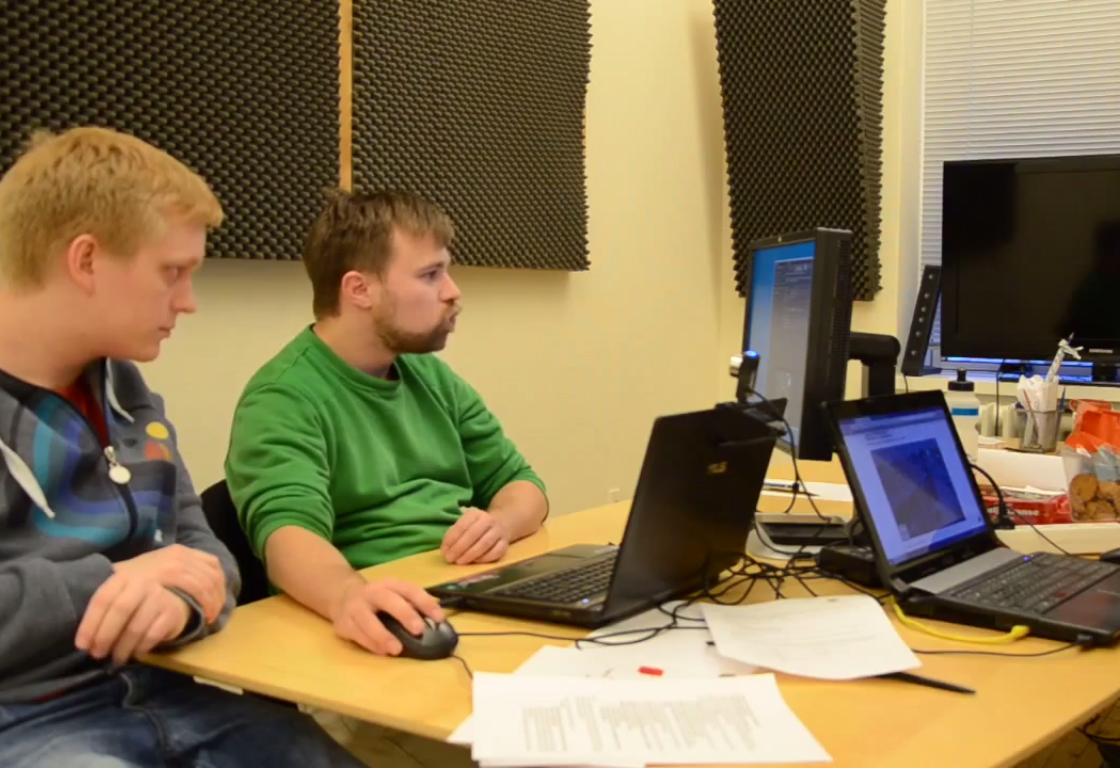
\includegraphics[width=0.3\textwidth]{Pics/test_setup}
\caption{The test participant used had two monitors at his disposal while working with the tool.}
\label{fig:framingConcept}
\end{figure}

\subsubsection{Basic Navigation}
The participants and facilitator sat down at another laptop with a second monitor connected. Here the facilitator gave the participant a basic introduction to Unity so that all participants had no problem understanding the Unity workspace layout, moving around with the scene view camera, changing the position and rotation of objects, etc. To ensure this, the participants was told to move the scene view camera to three positions in the scene (e.g. move camera above the green cube in Figure \ref{fig:sceneAll}). The participant was tasked to move the camera to three specific locations in the environment to ensure they felt comfortable in the workspace. 

\subsubsection{Training} 
After this the facilitator introduced the camera tool to the participant, first he explained the concept using a printed out version of Figure \ref{fig:framingConceptNew}, then he opened the tool in Unity and explained its features and functionalities. The participant tried each feature as they were introduced, e.g. when the facilitator explained how to place influence points and how to connect them, the participant was asked to try it for themselves. 

\subsubsection{Tasks}
When all features were explained, the participant was handed a piece of paper with five tasks. The tasks are as follows:

\begin{enumerate}[noitemsep,nolistsep]
\item Make the camera's field of view change.
\item Make the camera tilt upwards.
\item Make the camera look at the tall pink cylinder.
\item Make the camera go from a low perspective to bird’s-eye view.
\item Change the interpolation of one of the previous assignments by changing the animation curve.
\end{enumerate} 

The chosen tasks reflects five common features and tasks that's often used when setting up a framing and a camera interpolation. The participant had to solve the tasks themselves, the facilitator only intervened when the participant was struggling with something, asked a question, or at unforeseen occurrences (e.g. bugs). 

\subsubsection{Creative}
After this, the participant was introduced to a level with a modelled environment. They were then tasked to envision and sketch two ways for the camera to move as the play character moved through this environment, when they had two ideas, they were tasked to implement both of these using our camera tool. The facilitator remained as neutral as possible for this part of the test, but still intervened if they participant was struggling or encountered things like bugs.

\subsubsection{Post-test Questionnaire}
Finally, the participant went back to the first laptop and answered a post-test questionnaire. The participant was thanked and the test ended.
\subsubsection{Materials}
Three scenes was constructed for the test. The first was an environment with simple geometry scene. The second was used in the first part of the test when participants were introduced to the camera tool and had to complete 5 tasks. The third level was for the creative part of the test when participants had to envision the camera movement in an environment and then implement it. 

\begin{figure*}[htbp]
\centering
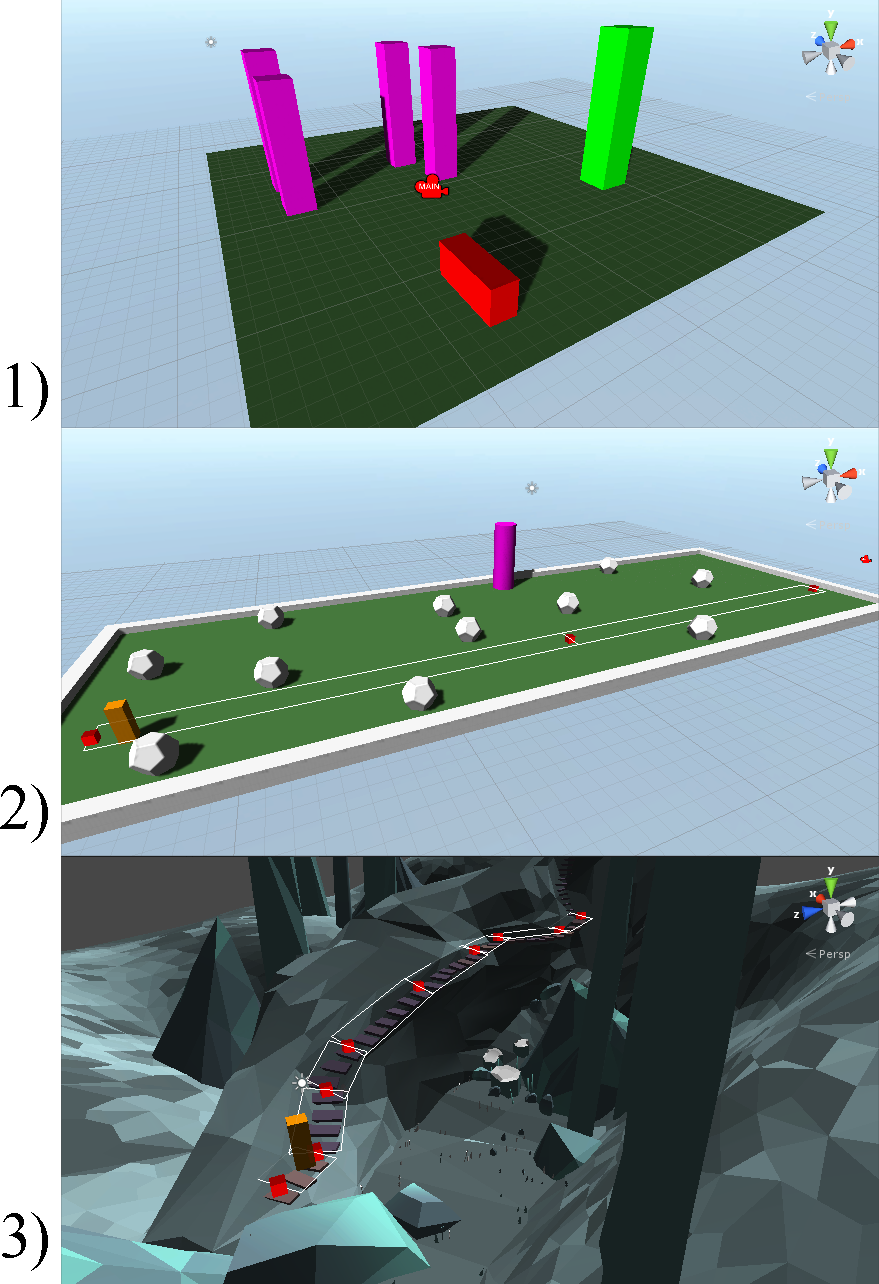
\includegraphics[width=0.45\textwidth]{Pics/sceneAll}
\caption{1) The participant was instructed to move the camera to the top of the green cube, between the purple pillars and to the bottom of the red cube and then rotate the camera to look at the purple pillars. 2) A flat plane with simple geometry to make it easier to see differences when changing camera settings. 3) A mountainous environment with a staircase attached to the mountainside.}
\label{fig:sceneAll}
\end{figure*}
\subsection{Evaluation Questionnaire}
The participants had varied experience with Autodesk Maya, ranging from six months to six years. In Unity, their experience ranged from none at all to more than a year.

The participants rated their agreement with a list of statements using a 5-point Likert scale ranging from ``strongly disagree" to ``strongly agree". 

%While the test participants tried the FCT, they were recorded  their two monitors were. Additionally, a webcam recorded the face of the participants, together with the audio. An observer wrote notes during the evaluation. For the questionnaire, the participants rated themselves on the following statements using a 5-point Likert scale ranging from "strongly disagree" to "strongly agree". 
%\begin{itemize}[noitemsep,nolistsep]
%\item \textit{I felt empowered using this tool.}
%\item \textit{I felt restricted using this tool.}
%\item \textit{I felt I got the tasks done quickly.}
%\item \textit{I felt the tool allowed me to complete the tasks well.}
%\end{itemize}

When asked if the participants \textit{``felt empowered using the tool"}, four participants \textit{agreed}, while the remaining two \textit{strongly agreed}. When asked if they \textit{``felt restricted using the tool"}, five participants \textit{disagreed} while the remaining participant \textit{strongly disagreed}. When asked they if they felt that they \textit{``got the tasks done quickly"}, four participants \textit{agreed} and two \textit{strongly agreed}. To find out how effective the participants felt using our tool, we asked them if they \textit{``felt the tool allowed them to complete the tasks well"}, three participants \textit{agreed} and three \textit{strongly agreed}.

%To find out how efficient the participants felt using the FCT, we asked them if they felt they \textit{"got the tasks done quickly"}. Four participants \textit{agreed} and two \textit{strongly agreed}. To find out how effective the participants felt using our tool, we asked them if they \textit{"felt the tool allowed them to complete the tasks well"}. Three participants \textit{agreed} and three \textit{strongly agreed}.

Furthermore, they were asked whether they preferred the \textit{be the camera} or the \textit{snapshot} feature for adjusting cameras. Four chose \textit{ be the camera} and two chose \textit{snapshot}. 
They were also asked how useful they thought the preview features were. The response choices were ``not useful", ``somewhat useful", ``very useful", ``didn't use any of them", and ``don't know". Five participants found them \textit{very useful}, and one found it \textit{somewhat useful}.
Finally, the participants were asked what their overall favorite feature was. Three participants noted the \textit{be the camera} feature as their overall favourite feature, while the \textit{slider preview} was the favourite for the other three participants. 

To see the full demographic and evaluation questionnaire, see the attached worksheets.

%When asked about the preview features, five participants found them \textit{very useful}, and one found it \textit{somewhat useful}. The participants were also asked whether they preferred the \textit{be the camera} or the \textit{snapshot} feature. Four named\textit{ be the camera} and two named \textit{snapshot}. Furthermore, three participants noted the \textit{be the camera} feature as their overall favourite feature, while the \textit{slider preview} was the favourite for the other three participants. 

%Furthermore, they were asked whether they preferred the \textit{be the camera} or the \textit{snapshot} feature for adjusting cameras. They were also asked how useful they thought the preview features were. The response choices were "not useful", "somewhat useful", "very useful", "didn't use any of them", and "don't know". To highlight the best features in the tool, the participants were asked to name their favourite feature from a list of 7.

%When asked about the preview features, five participants found them \textit{very useful}, and one found it \textit{somewhat useful}. The participants were also asked whether they preferred the \textit{be the camera} or the \textit{snapshot} feature. Four named\textit{ be the camera} and two named \textit{snapshot}. Furthermore, three participants noted the \textit{be the camera} feature as their overall favourite feature, while the \textit{slider preview} was the favourite for the other three participants. 
%\subsubsection{Data Analysis}
The video recordings from the experiment was coded internally at a later date in pairs of two. The two pairs coded one participant in unison and then split up and worked in parallel. Repeated ideas, events and observations was tagged with certain tags. The tags used are \textit{confusion}, \textit{exploration}, and \textit{problem}.

An event was tagged with \textit{confusion} if a participant was confused that a feature didn't work as they expected or struggled doing what they wanted/envisioned (e.g. did not connect influence points; unsure why interpolation didn't not function properly), 
\textit{exploration} means that a participant explored the interface or features of the camera tool by themselves without prompting them or if they asked questions about the features (e.g. \textit{"What consequence does it have if the points are not connected? Would that be a cut?"}), 
%\textit{observation} is an (subjective) observation made internally about the participant and their behavior or approach to the tasks (e.g. no problem navigating in Unity), 
\textit{problem} means a participant got stuck or encountered a problem so they could not progress (e.g. tried changing position of camera while Aim Point was active. The camera jumped around seemingly random in the scene and moved to an unwanted position because of it.)
%\subsection{Results} \label{results}
Four participants reported to have between one and three years of experience with Autodesk Maya, another had between four and six years of experience and the last had seven or more years of experience. Only one participant had more than one year of experience with Unity, another had between six and twelve months of experience with it, the rest reported to have less than six months of experience.
When asked if they \textit{'felt empowered using the tool'}, 2/6 participants \textit{strongly agreed} and 4/6 participants \textit{agreed}.

Coded data shows...



When asked if the participants felt empowered using the tool, four participants agreed while the remaining two strongly agreed. When asked if the they felt restricted when using the tool, five participants disagreed while the remaining participant strongly disagreed. To find out how efficient the participants felt using our tool, we asked them if they felt they got the tasks done quick, four participants agreed and two strongly agreed. To find out how effective the participants felt using our tool, we asked them if they felt the tool allowed them to complete the tasks well, three participants agreed and three strongly agreed.
When asked about the preview features, five participants found them very useful, and one found it somewhat useful. For the participants' favorite feature for adjusting camera positions, four named 'Be the camera' and two named 'Snapshot' as their favorite. Furthermore, three participants noted the 'Be the camera' feature as their overall favorite while the 'Slider Preview' was the favorite for the other three participants. 
%\subsection{Observations}
Quotes, etc...